% Includable chapter. Packages: amsmath, amssymb, graphicx, booktabs, hyperref.
% Keep the accompanying figures folder relative to the main document.
% Earlier-chapter references resolve normally in the complete notes.
% The standalone wrapper supplies descriptive text instead of absent numbers.
\providecommand{\QRMTprevious}[3]{#2~\ref{#1}}
\chapter{From observations to evidence}
\label{chap:data-science}
\begin{center}\large Patterns, predictions, and uncertainty\end{center}

\begin{center}
\begin{minipage}[t]{0.47\textwidth}
\centering\vspace{0pt}
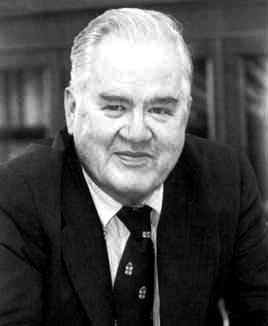
\includegraphics[height=1.15in]{images/tukey.jpeg}\\[5pt]
\small ``Far better an approximate answer to the right question
\ldots\ than an exact answer to the wrong question''\\[3pt]
---John W. Tukey (1915--2000)\\
\scriptsize \href{https://doi.org/10.1214/aoms/1177704711}
{\emph{The Future of Data Analysis} (1962), pp.~13--14; excerpt.}
Photograph: \href{https://mathshistory.st-andrews.ac.uk/Biographies/Tukey/pictdisplay/}{MacTutor History of Mathematics}.
\end{minipage}\hfill
\begin{minipage}[t]{0.47\textwidth}
\centering\vspace{0pt}
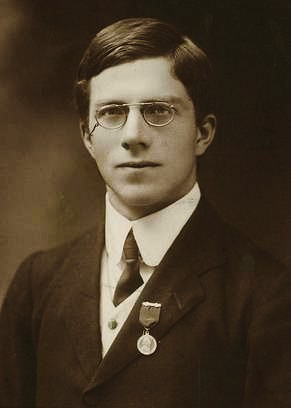
\includegraphics[height=1.15in]{images/fisher.jpg}\\[5pt]
\small ``To consult the statistician after an experiment is finished
is often merely to ask him to conduct a post mortem examination.''\\[3pt]
---R. A. Fisher (1890--1962)\\
\scriptsize \href{https://gwern.net/doc/statistics/decision/1938-fisher.pdf}
{Presidential Address, Indian Statistical Congress (1938), p.~17.}
Photograph: 1913, unknown photographer;
\href{https://commons.wikimedia.org/wiki/File:Youngronaldfisher2.JPG}{Wikimedia Commons}.
\end{minipage}
\end{center}


How long will we wait at the cafeteria? How many people will use a new
bus service? Does a different way of explaining a problem help students
solve it? We cannot answer these questions by reasoning from definitions
alone. We need observations. Yet observations do not announce what they
mean: we must decide what to record, how to summarise it, and what
conclusions it can support.

Data science brings together measurement, mathematical models, and
computation to learn from observations. A calculation can be exact while
its conclusion about the world remains uncertain. The aim is to make that
uncertainty intelligible, so that we can reason and act with it.
All numerical datasets in this chapter are constructed teaching examples,
not findings about an actual campus or population.

\section{Begin with a question, then make a table}
\label{sec:ds-data}
\paragraph{The problem.}
A campus cafeteria wants to know how long customers wait between joining
the queue and receiving their food. What should be recorded, and what
would count as a useful answer?

An observation should correspond to one clearly specified event: a
customer's visit. We might record the date, joining time, serving time,
queue length on arrival, and whether the visit was during the lunch rush.
The waiting time is the difference between two times, expressed in minutes.
A row represents a visit and a column represents a variable.
\begin{center}
\begin{tabular}{ccccc}
\toprule
Visit & Joined & Served & Wait (minutes) & Lunch rush?\\
\midrule
1 & 12:10 & 12:12 & 2 & no\\
2 & 12:13 & 12:16 & 3 & no\\
3 & 13:02 & 13:26 & 24 & yes\\
\bottomrule
\end{tabular}
\end{center}

Not every number is a measurement. Visit 3 is an identifier; averaging
visit identifiers would tell us nothing about the queue. Waiting time is
numerical, while the lunch-rush indicator is categorical. A numerical
variable may count separate objects, or measure a quantity such as time
that can vary continuously. Recording time to the nearest minute does
not make the underlying waiting process occur in whole-minute jumps.

Before calculating, check the table. Are all waits in the same units?
Was a visit entered twice? Does a blank mean ``not recorded'' or ``zero''?
Does a customer who leaves before being served disappear from the data?
A long wait might be a recording error, but it might also be precisely the
experience we need to understand. Cleaning data requires decisions whose
reasons should be recorded.

The question also determines whose visits matter. If we want the experience
of a randomly chosen visit, frequent customers contribute more visits.
If we want the experience of a randomly chosen student, we need a different
sampling scheme. A table organised around visits does not automatically
answer questions about students: the unit of observation must match the
question we want to ask.

\section{A summary should preserve what matters}
\label{sec:ds-summaries}
Suppose ten recorded waits, in increasing order, are
\[
2,\ 3,\ 3,\ 4,\ 4,\ 4,\ 5,\ 5,\ 6,\ 24.
\]
Their \emph{mean} is
\[
\bar x=\frac{1}{n}\sum_{i=1}^{n}x_i=\frac{60}{10}=6.
\]
The \emph{median}, halfway between the two middle observations here, is
$4$ minutes. These answers differ because the long wait pulls the mean
upwards. The mean describes the average waiting time per visit; the median
identifies a point with at least half the observations on either side.
If the question is whether customers sometimes wait unacceptably long,
neither number is enough. In this sample, one of ten waits exceeds
10 minutes. Figure~\ref{fig:ds-waits} makes the isolated long wait
visible alongside the two summaries.

\begin{figure}[htbp]\centering
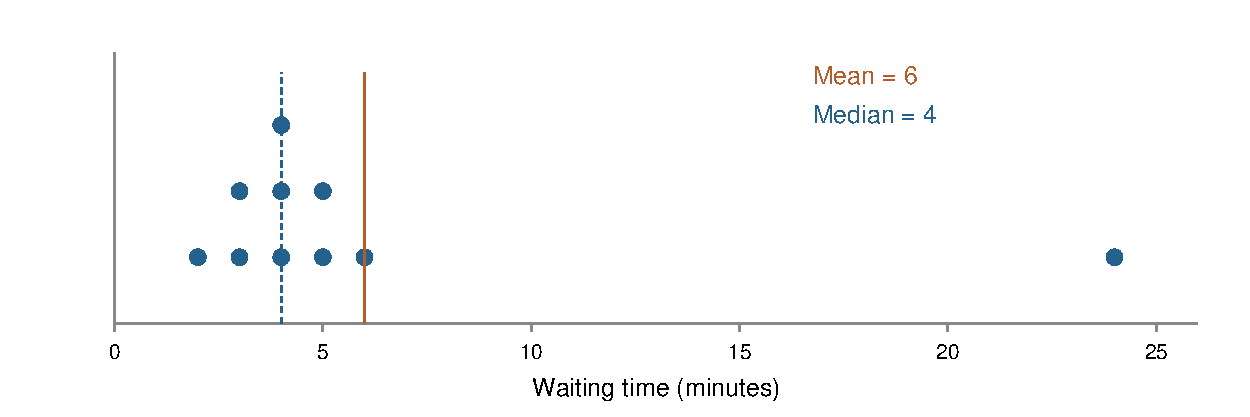
\includegraphics[width=0.85\textwidth]{figures/waits.pdf}
\caption{Ten observations shown individually. The mean and median answer
different questions; the isolated long wait should not disappear behind
an average. Stacked points represent repeated values.}
\label{fig:ds-waits}
\end{figure}

A useful measure of spread is the mean squared distance from the mean:
\[
 v=\frac1n\sum_{i=1}^{n}(x_i-\bar x)^2.
\]
Squaring prevents positive and negative deviations from cancelling.
The square root, $\sqrt v$, returns to the original units and is called a
standard deviation. This formula describes the displayed dataset. When
estimating population variance from a random sample, a common estimator
uses $n-1$ in the denominator instead; we will not need that correction
for our descriptive calculations.

\subsection{The mean as a geometric centre}
Place every observation on a number line, with one equal mass at each
observed value. Repeated values contribute repeated masses. The mean is
the \emph{balance point} of these masses: signed displacements from it
sum to zero,
\[
 \sum_{i=1}^n(x_i-\bar x)=\sum_{i=1}^n x_i-n\bar x=0.
\]
For our waiting times, the nine values at or below six contribute a total
signed displacement of $-18$ minutes; the single value 24 contributes
$+18$. They balance at six. A single distant observation can therefore
move this centre considerably, even though most observations lie elsewhere.

There is a second geometric characterisation. Suppose we want to replace
all the points by one representative point $c$. The distance from $x_i$
to $c$ is $|x_i-c|$. If we measure the total discrepancy by the sum of
\emph{squared} distances, then the mean is the best representative point.
For any $c$,
\[
 \sum_{i=1}^{n}(x_i-c)^2
 =\sum_{i=1}^{n}(x_i-\bar x)^2+n(c-\bar x)^2.
\]
To verify this, write $x_i-c=(x_i-\bar x)+(\bar x-c)$ and expand the
square. The cross terms sum to zero because the signed displacements
from $\bar x$ sum to zero. What remains is the displayed identity.

Its meaning is worth reading in words: the squared-distance cost of using
$c$ equals the cost of using the mean, plus a nonnegative penalty for
moving the representative point away from the mean. The penalty is zero
only at $c=\bar x$. Thus the mean is the \emph{least-squares centre} of
points on a line. ``Centre'' depends on our choice of discrepancy: if we
minimise the sum of absolute distances instead, a median is a minimiser.
Figure~\ref{fig:ds-mean-geometry} shows both the balance-point and
least-squares interpretations.

\begin{figure}[htbp]\centering
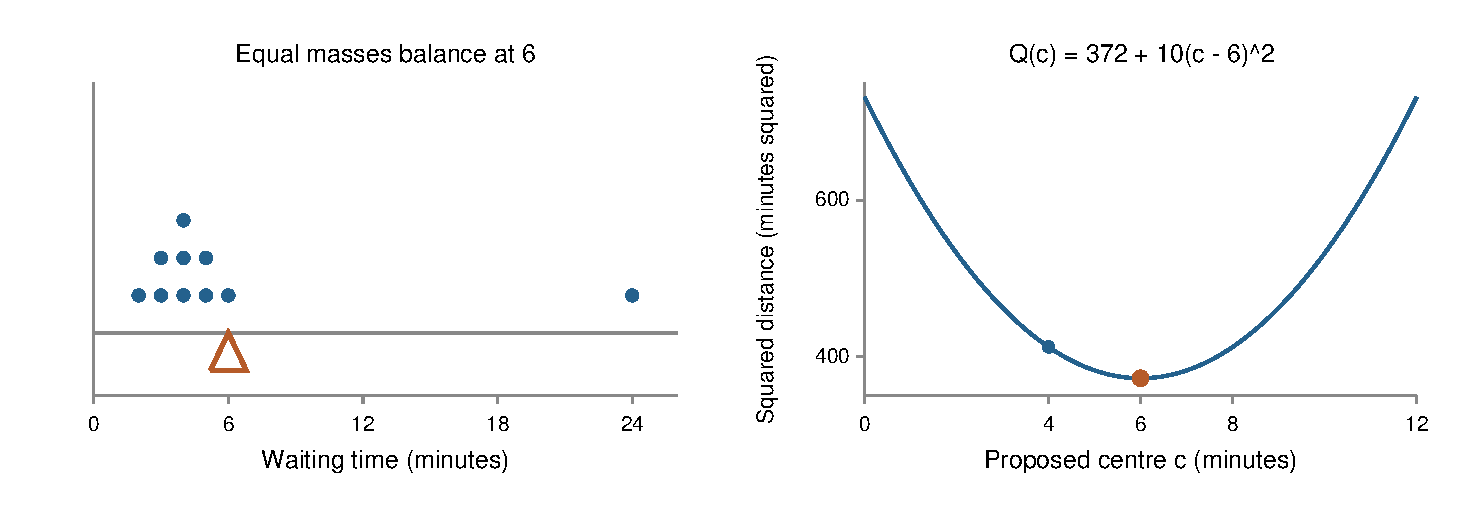
\includegraphics[width=\textwidth]{figures/mean-geometry.pdf}
\caption{Left: equal masses at the ten waiting times balance at six.
Right: the total squared distance $Q(c)$ is smallest at the same point.
For these data $Q(c)=372+10(c-6)^2$; moving the proposed centre from six
to four increases the cost by 40 square minutes.}
\label{fig:ds-mean-geometry}
\end{figure}

Later we will replace a cloud of points in a plane by a line rather than
replace points on a number line by a single centre. The same question
will guide the choice: which line makes the chosen squared distances
as small as possible?

\section{From a collection of values to a probability distribution}
\label{sec:ds-distributions}
\paragraph{The problem.}
Instead of asking only for an average wait, we want to describe which
waits are possible and how likely they are. How can one mathematical
object express both?

Imagine selecting one of the ten recorded visits uniformly at random,
so that each visit has probability $1/10$. Let $X$ be its waiting time.
The probability that $X=4$ is $3/10$, because three visits have that wait.
The table of values and their probabilities is a \emph{probability
distribution}. It describes the uncertainty in $X$ before the visit is
selected. A quantity whose value depends on a random outcome is called
a \emph{random variable}.

The distribution constructed by assigning probability $1/n$ to each
recorded observation is the \emph{empirical distribution}. It describes
the data we have. Treating it as a description of future visits is a further
modelling step: tomorrow's staffing or demand might be different.

\paragraph{Ten observations are not a population distribution.}
Only one of our ten visits lasted more than ten minutes. Its empirical
probability is therefore $1/10=0.1$, but the population probability need
not be exactly $0.1$. An eleventh long wait would change the empirical
fraction to $2/11$. If no long waits had appeared, that would not establish
that long waits are impossible. Small samples are especially poor at
revealing rare events or the far ends of a distribution.

Even a large sample can mislead if it contains only quiet mornings while
our question concerns the entire week. Estimating a distribution requires
attention both to how many observations we have and to how they were
selected. We will return to these issues when discussing sampling.

\subsection{Probability: frequencies and axioms}
A \emph{frequentist interpretation} connects probability with the relative
frequency of an event in many repetitions under stable conditions. For
example, if a model assigns probability $0.1$ to a wait longer than ten
minutes, it predicts that the fraction of such waits will tend to be close
to $0.1$ in a sufficiently large collection of independent visits governed
by that model. It does not require exactly one long wait in every ten,
or guarantee that a growing sample's fraction moves steadily towards $0.1$.

Observed frequencies can therefore be used to estimate probabilities,
but a finite observed fraction and the probability being estimated are
different objects.

\paragraph{What the law of large numbers says.}
Suppose observations are independent, come from the same distribution,
and have a finite mean $\mu$ and finite variance. Independence means that
knowing one outcome does not change the probabilities for the others.
One version of the \emph{law of large numbers} says that, for any fixed
tolerance $\varepsilon>0$,
\[
 P\bigl(|\bar X_n-\mu|>\varepsilon\bigr)\longrightarrow0
 \qquad\text{as }n\longrightarrow\infty.
\]
In words: with a sufficiently large sample, its average is very likely
to be close to the population mean. To apply this to long waits, record
1 for a wait exceeding ten minutes and 0 otherwise. Their sample mean
is the observed fraction of long waits, and their population mean is
the probability of a long wait. The same law therefore justifies using
frequencies to estimate probabilities.\footnote{For an explanation and
proof, see Hossein Pishro-Nik, \emph{Introduction to Probability, Statistics,
and Random Processes},
\href{https://www.probabilitycourse.com/chapter7/7_1_1_law_of_large_numbers.php}
{Section 7.1.1, ``Law of Large Numbers''}. The finite-variance assumptions
used here give a convenient elementary version of the weak law.}

This is a statement about the chance of an inaccurate average, not a
promise that each additional observation improves it. Individual waits
remain variable; it is the average that becomes more stable. Nor does
a run of short waits make a long wait ``due'' under the independent model.
If all observations come from quiet mornings, the law can stabilise an
estimate for quiet mornings; it cannot turn it into an estimate for the
whole week. Section~\ref{sec:ds-sampling} shows how the spread of sample
means decreases under these assumptions.

The \emph{axiomatic approach} begins with rules for assigning probabilities.
Let $\Omega$ be the set of possible outcomes, called the sample space.
An \emph{event} $A$ is a specified collection of outcomes: for example,
``the selected visit has a wait longer than ten minutes''. The basic rules
are:
\begin{enumerate}
\item $P(A)\geq0$: probabilities are nonnegative.
\item $P(\Omega)=1$: some outcome in the sample space must occur.
\item If $A$ and $B$ cannot both occur, then
$P(A\cup B)=P(A)+P(B)$: add probabilities of mutually exclusive events.
The rule also holds for a countable collection of pairwise disjoint events.
\end{enumerate}
These rules imply, for example, that $P(\text{not }A)=1-P(A)$.
They do not say that every outcome is equally likely. That is a separate
assumption which may or may not be appropriate.

\begin{center}
\begin{minipage}{\textwidth}
\begin{minipage}[c]{0.23\textwidth}
\centering
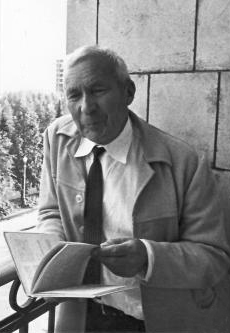
\includegraphics[height=1.25in]{images/kolmogorov.jpg}
\end{minipage}\hfill
\begin{minipage}[c]{0.72\textwidth}
\small ``The theory of probability \ldots\ can and should be developed
from axioms in exactly the same way as Geometry and Algebra.''\\[4pt]
---Andrey Kolmogorov (1903--1987)\\[3pt]
\scriptsize \href{https://mathematik.com/Kolmogorov/}
{\emph{Foundations of the Theory of Probability}, preface (1933);
English translation, excerpt.} Photograph by Konrad Jacobs,
Oberwolfach Photo Collection, via
\href{https://commons.wikimedia.org/wiki/File:Andrej_Nikolajewitsch_Kolmogorov.jpg}{Wikimedia Commons};
\href{https://creativecommons.org/licenses/by-sa/2.0/de/}{CC BY-SA 2.0 DE}.
\end{minipage}
\end{minipage}
\end{center}

Frequency and axioms are not competing methods for computing the same
number. The first gives an interpretation and a route from observations
to estimates; the second supplies a mathematical framework once a
probability model has been specified. A frequency estimate can obey all
the axioms yet describe the population poorly. Conversely, the axioms
alone cannot tell us the cafeteria's chance of a long wait. We need
observations and an argument for using them in the proposed setting.

\subsection{A discrete model of waiting}
Consider a deliberately simplified model, chosen for easy calculations:
\begin{center}
\begin{tabular}{c rrrr}
\toprule
Wait $x$ (minutes) & 0 & 5 & 10 & 20\\
Probability $P(X=x)$ & 0.1 & 0.4 & 0.4 & 0.1\\
\bottomrule
\end{tabular}
\end{center}
These probabilities are not fitted to the ten visits above. They specify
a separate hypothetical model. Each probability is nonnegative, and their
sum is one: some possible outcome must occur. To find the probability of
an event, add the probabilities of its outcomes. Thus
\[
 P(X\leq5)=0.1+0.4=0.5,\qquad P(X>10)=0.1.
\]
The \emph{expected value} is the probability-weighted mean,
\[
 \mu=\mathbb E[X]=\sum_x xP(X=x)
 =0(0.1)+5(0.4)+10(0.4)+20(0.1)=8.
\]
An expected wait of eight minutes does not mean that an eight-minute wait
is possible in this model. It is the long-run average predicted for many
independent visits governed by this distribution.

The model's variance and standard deviation are
\[
 \sigma^2=\mathbb E[(X-\mu)^2]=26,
 \qquad \sigma=\sqrt{26}\approx5.10\text{ minutes}.
\]
The distribution can support different decisions. A customer allowing
five minutes faces a different risk from one allowing ten. A manager
concerned about very long waits needs the upper tail, not just $\mu$.

\subsection{Continuous measurements: probability is area}
For a continuously varying measurement, it is often more useful to assign
probabilities to intervals. A \emph{probability density} $f(x)$ is a
nonnegative curve whose total area is one. The probability of an interval
is the area under the curve over that interval. A height on the graph is
not itself a probability.

For example, suppose a bus arrives exactly every ten minutes and a
passenger's arrival is uniformly spread over one interval between buses.
Their waiting time is modelled by a uniform distribution on $[0,10]$.
The density is $1/10$ per minute throughout this interval, so
\[
 P(2\leq X\leq5)=(5-2)\frac1{10}=0.3.
\]
In this ideal continuous model, any exact single value has probability
zero; intervals can nevertheless have positive probability. Real recording
rounds measurements, and ``five minutes'' may denote a whole interval.
The uniform model would be inappropriate if passengers consulted the
schedule and deliberately arrived just before a bus.
Figure~\ref{fig:ds-distributions} contrasts the two models: a bar height
is a probability on the left, whereas an area is a probability on the right.

\begin{figure}[htbp]\centering
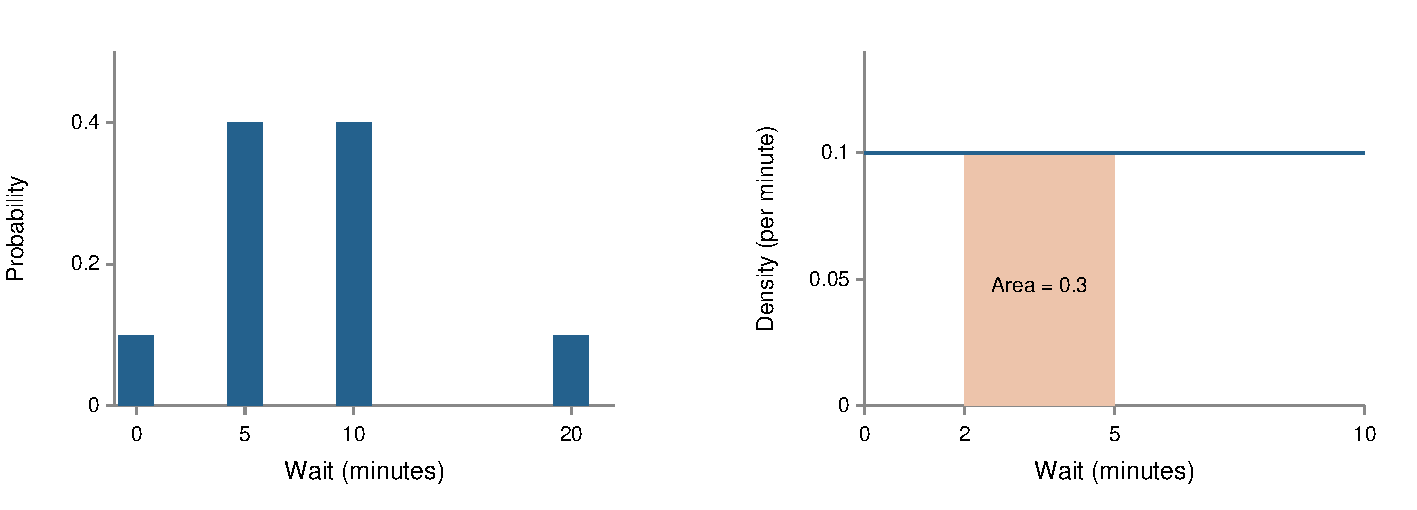
\includegraphics[width=\textwidth]{figures/distributions.pdf}
\caption{Left: probabilities assigned to individual outcomes in the
discrete waiting model. Right: a density for a continuous uniform wait.
The shaded rectangle has area $0.3$, the probability of waiting between
two and five minutes. The vertical axes have different meanings.}
\label{fig:ds-distributions}
\end{figure}

\subsection{A few important families of distributions}
\label{sec:ds-standard-distributions}
The uniform distribution above is one useful model. Other recurring kinds
of questions lead to other families. Choosing a distribution means making
assumptions about how observations arise; it is not merely choosing a
convenient formula.

\begin{center}
\begin{minipage}{\textwidth}
\begin{minipage}[t]{0.47\textwidth}
\centering
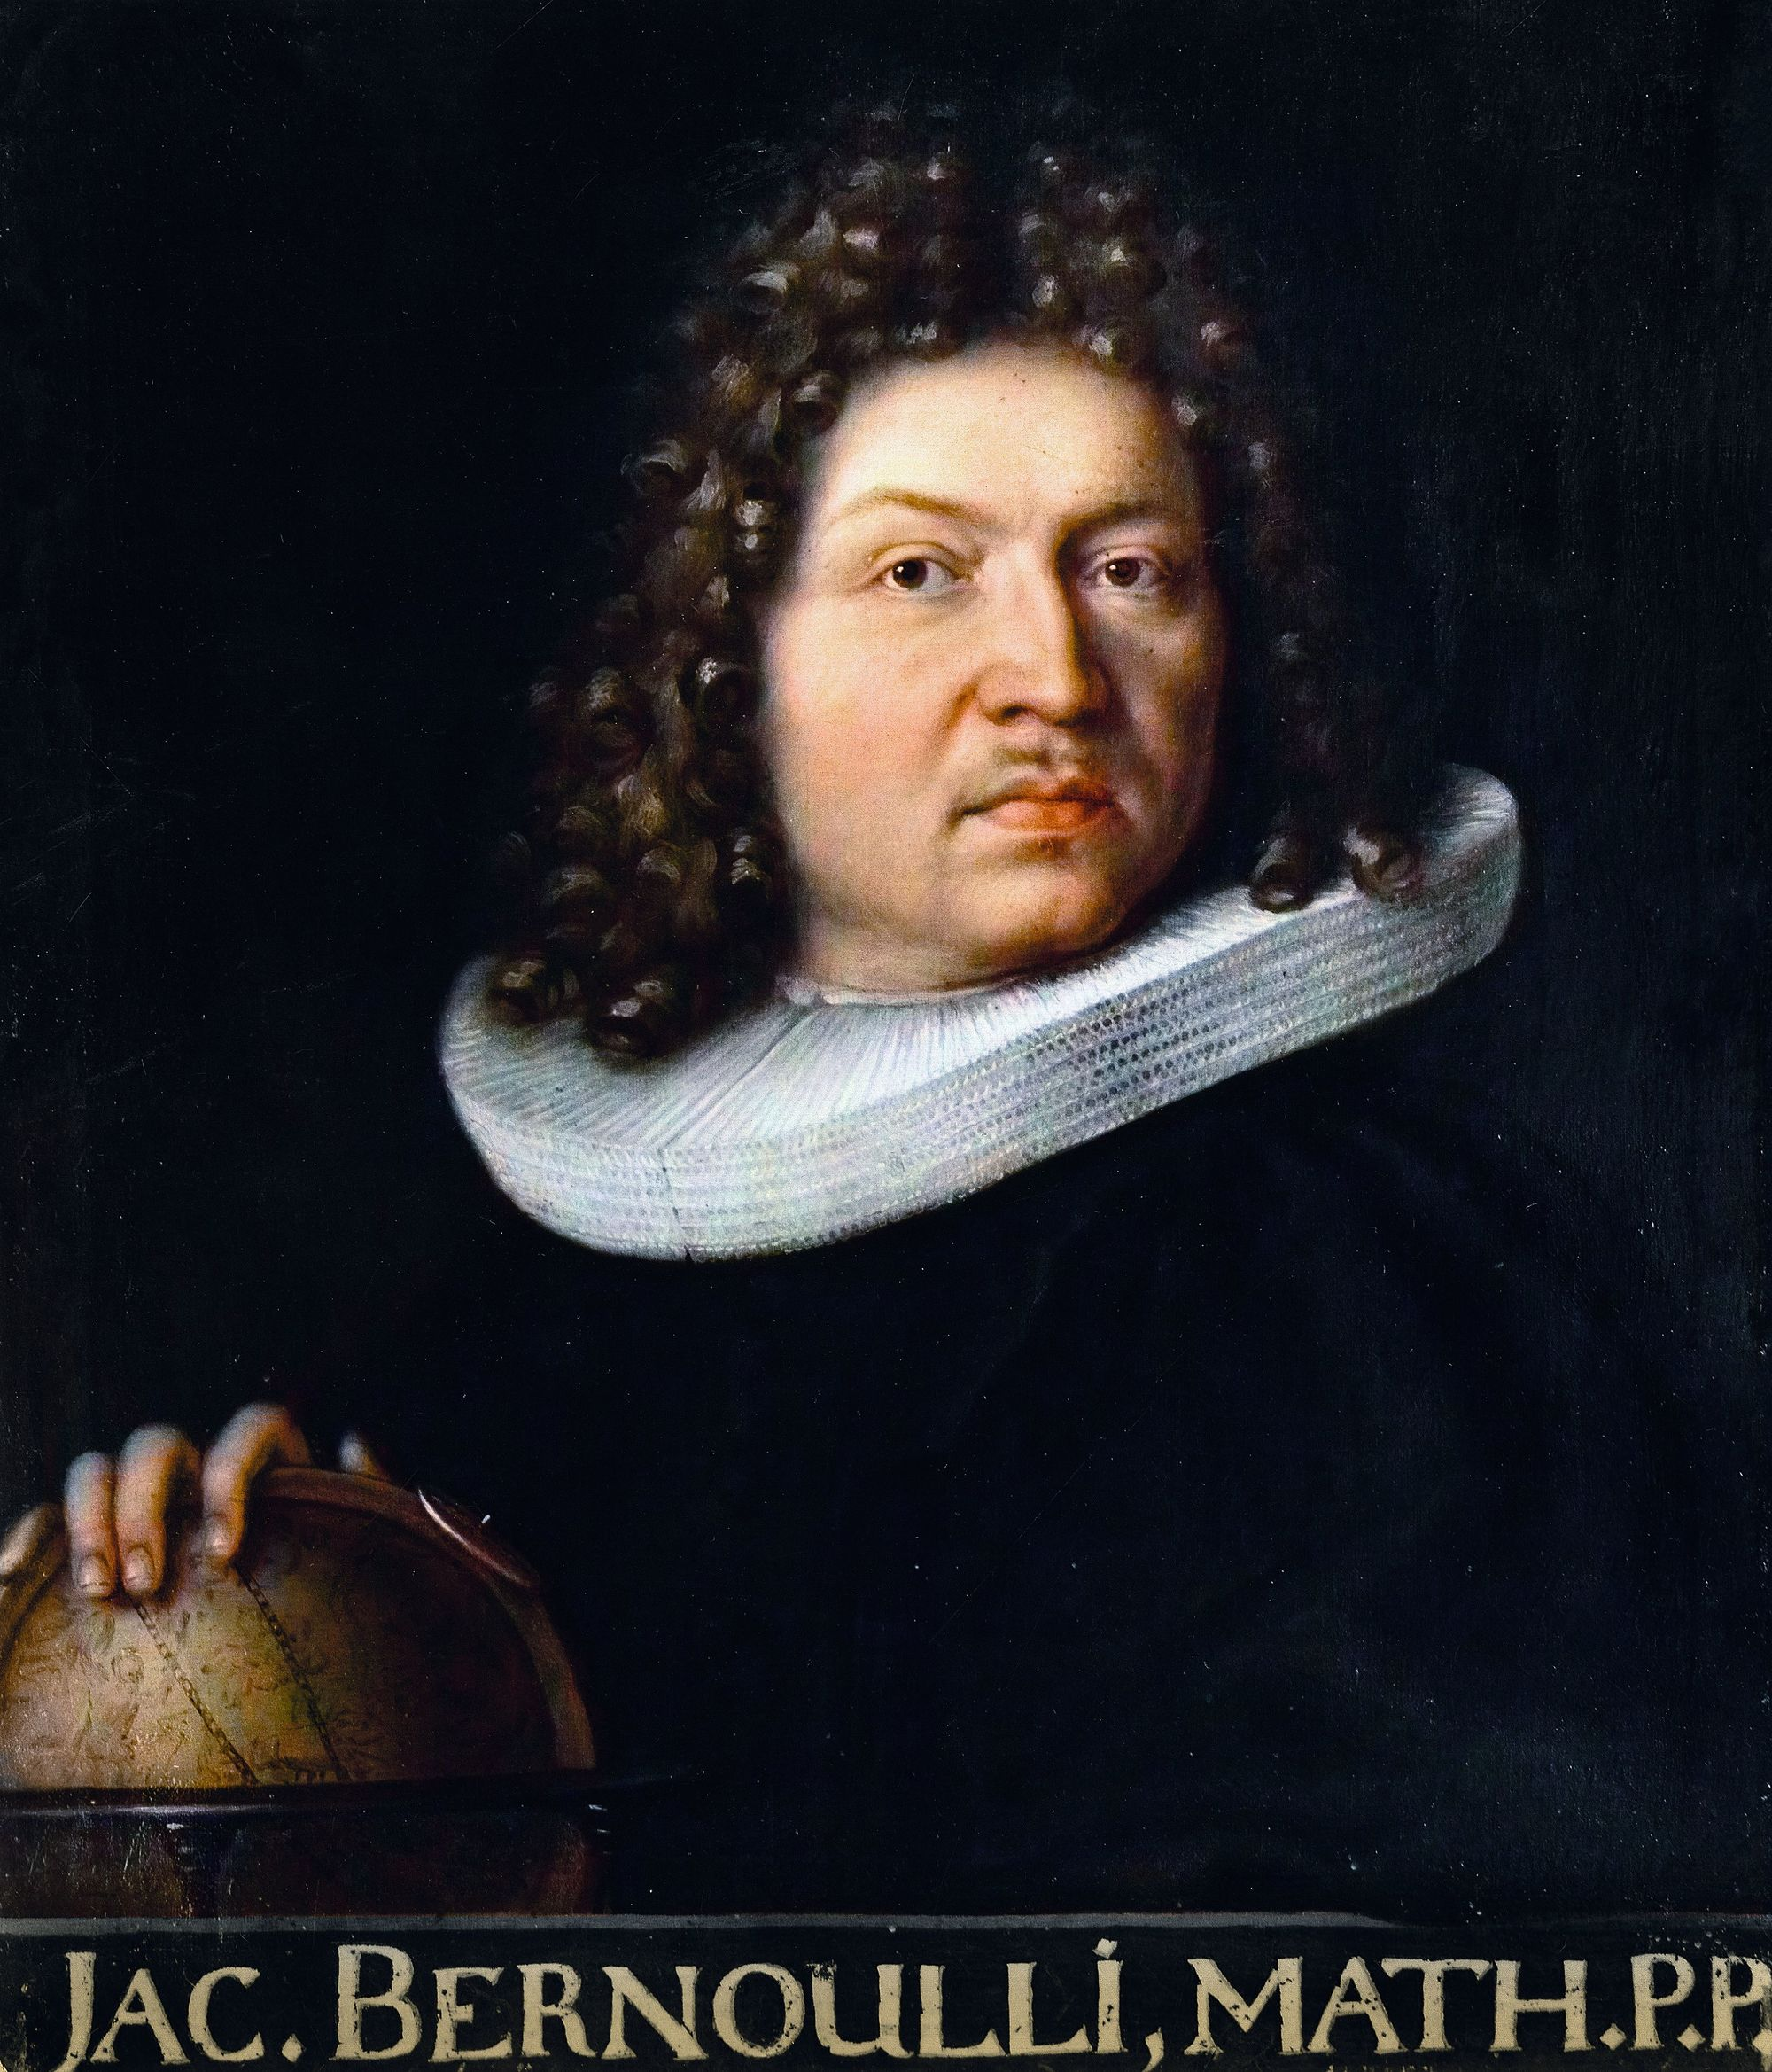
\includegraphics[height=1.15in]{images/bernoulli.jpg}\\[4pt]
\small\textbf{Jacob Bernoulli (1655--1705)}\\[3pt]
His \emph{Ars Conjectandi}, published posthumously in 1713, developed
probability theory and the law of large numbers.\\[3pt]
\scriptsize Portrait by Niklaus Bernoulli (1687),
\href{https://commons.wikimedia.org/wiki/File:Jakob_Bernoulli.jpg}{Wikimedia Commons}; public domain.
\end{minipage}\hfill
\begin{minipage}[t]{0.47\textwidth}
\centering
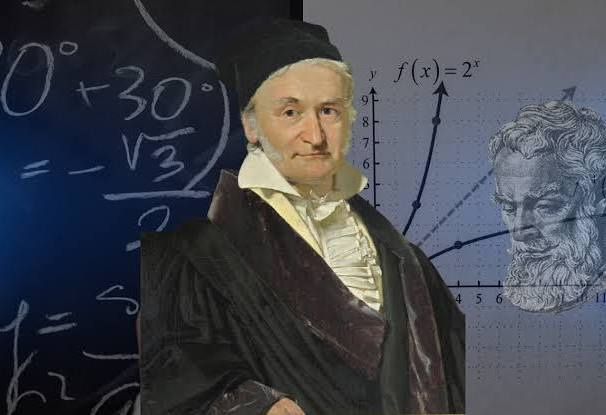
\includegraphics[height=1.15in]{images/gauss2.jpg}\\[4pt]
\small\textbf{Carl Friedrich Gauss (1777--1855)}\\[3pt]
His work connected measurement errors with least squares and the normal
distribution. The distribution had appeared earlier in de Moivre's work.\\[3pt]
\scriptsize Portrait by C. A. Jensen (1840),
\href{https://commons.wikimedia.org/wiki/File:Carl_Friedrich_Gauss_1840_by_Jensen.jpg}{Wikimedia Commons}; public domain.
\end{minipage}
\end{minipage}
\end{center}

\paragraph{Bernoulli: one yes-or-no outcome.}
Let $X=1$ if a customer's wait exceeds ten minutes and $X=0$ otherwise.
If the probability of a long wait is $p$, then
\[
 P(X=1)=p,\qquad P(X=0)=1-p.
\]
This is a \emph{Bernoulli distribution}, with mean $p$ and variance
$p(1-p)$. It models a single binary outcome: a long wait, a defective item,
or a yes answer in a survey. Averaging these zero-or-one observations gives
the proportion of yes outcomes.

\paragraph{Binomial: how many yes outcomes?}
For $n$ independent Bernoulli observations with the same probability $p$,
their sum $K$ has a \emph{binomial distribution}:
\[
 P(K=k)=\binom nk p^k(1-p)^{n-k},\qquad k=0,1,\ldots,n.
\]
Its mean is $np$. If the chance of a long wait is $0.1$, the model predicts
an average of two long waits among 20 independent visits, not exactly two
in every sample. It is useful for counts and proportions; we will meet
it again when counting wins in Section~\ref{sec:ds-inference}.

Figure~\ref{fig:ds-bernoulli-binomial} compares the outcome of a single
trial with the count over 20 independent trials. In both panels, the bar
heights are probabilities; their sum is one.

\begin{figure}[p]\centering
\includegraphics[width=0.88\textwidth]{figures/bernoulli.pdf}\\[5pt]
\includegraphics[width=0.88\textwidth]{figures/binomial.pdf}
\caption{Bernoulli and binomial distributions with $p=0.1$. The first
models one yes-or-no outcome; the second counts yes outcomes in 20
independent trials with the same probability.}
\label{fig:ds-bernoulli-binomial}
\end{figure}

\paragraph{Poisson: arrivals in a fixed interval.}
A \emph{Poisson distribution} models a count $K$ with
\[
 P(K=k)=e^{-\lambda}\frac{\lambda^k}{k!},\qquad k=0,1,2,\ldots.
\]
Here $\lambda>0$ is the expected count. For example, arrivals at a cafeteria
might be modelled this way over a quiet five-minute interval. The model
is appropriate when arrivals occur independently at a roughly constant
rate; friends arriving in groups or a sudden lunchtime rush can violate
these assumptions. It is widely used for arrival and event counts.

\paragraph{Gaussian: variation around a centre.}
The \emph{normal}, or \emph{Gaussian}, distribution has the symmetric
bell-shaped density
\[
 f(x)=\frac{1}{\sigma\sqrt{2\pi}}
       e^{-(x-\mu)^2/(2\sigma^2)},\qquad -\infty<x<\infty.
\]
Its mean $\mu$ locates the centre and its standard deviation $\sigma>0$
sets the spread. About 68\% of its probability lies within one standard
deviation of the mean, and about 95\% within two. Measurement errors can
sometimes be modelled this way, although a bell shape must not simply be
assumed. In particular, nonnegative, strongly skewed waiting times need
not be Gaussian.

A major reason for its importance is the \emph{central limit theorem}:
for independent observations from the same distribution with finite,
nonzero variance, the distribution of their mean, centred and scaled by
its standard error, approaches the standard normal distribution as the
sample grows. Thus sample means can be approximately Gaussian even when
individual observations are not. This explains the usefulness of normal
approximations in estimation, including the factor $1.96$ in
Section~\ref{sec:ds-estimation}: a normal distribution places 95\% of its
probability within $1.96$ standard deviations of its mean. The approximation
may require large samples, especially for highly skewed observations.

Figure~\ref{fig:ds-poisson-gaussian} contrasts an event count with a
continuous measurement. The Poisson plot shows probability at each integer;
the Gaussian plot shows a density, whose shaded area is approximately
$0.95$. Its parameters here are $\mu=0$ and $\sigma=1$: this is the
\emph{standard normal distribution}.

\begin{figure}[p]\centering
\includegraphics[width=0.88\textwidth]{figures/poisson.pdf}\\[5pt]
\includegraphics[width=0.88\textwidth]{figures/gaussian.pdf}
\caption{A Poisson distribution with expected count four, and the standard
normal distribution. The Poisson distribution has a small tail beyond the
displayed counts. In the Gaussian panel, the area between $-1.96$ and
$1.96$ is approximately 95\% of the total area.}
\label{fig:ds-poisson-gaussian}
\end{figure}

\subsection{Sampling from a specified distribution}
\label{sec:ds-sampling-algorithm}
\paragraph{The problem.}
Given distinct values $x_1,\ldots,x_m$ and probabilities
$p_1,\ldots,p_m$, how can we generate an observation that equals $x_i$
with probability $p_i$? Here the distribution is specified in advance:
we are generating data from a model, rather than collecting observations
from a population.

Assume we can draw a number $u$ uniformly from $[0,1)$. Partition this
interval into consecutive pieces of lengths $p_1,\ldots,p_m$, and return
the value assigned to the piece containing $u$. For our waiting-time model:
\begin{center}
\begin{tabular}{rrl}
\toprule
Wait (minutes) & Probability & Assigned interval\\
\midrule
0 & 0.1 & $[0,0.1)$\\
5 & 0.4 & $[0.1,0.5)$\\
10 & 0.4 & $[0.5,0.9)$\\
20 & 0.1 & $[0.9,1)$\\
\bottomrule
\end{tabular}
\end{center}
Thus $u=0.73$ produces a waiting time of ten minutes. The half-open
intervals ensure that a boundary point belongs to exactly one piece.

\paragraph{From the post-condition to the invariant.}
Define the cumulative probabilities
\[
 C_0=0,\qquad C_i=\sum_{j=1}^{i}p_j.
\]
The desired final assertion is $C_{i-1}\leq u<C_i$: we have found the
interval containing $u$. Following the method in
\QRMTprevious{sec:imperative-invariants}{Section}{the discussion of loop
invariants in the imperative computation chapter}, generalise this assertion
by keeping its lower inequality while allowing the upper one to remain
unsatisfied. Search from left to right, storing the current upper endpoint
$C_i$ in a variable $c$. Our invariant is
\[
 1\leq i\leq m,\qquad c=C_i,\qquad C_{i-1}\leq u<1.
\]
We need not store all the cumulative probabilities: $c$ is updated as the
search proceeds. The bound function is the nonnegative integer $m-i$.

\begin{quote}
\begin{minipage}{\linewidth}
\textbf{Procedure: Sample from a finite distribution}\\[4pt]
\textit{// Pre-condition: $m\geq1$; the $x_i$ are distinct;}\\
\textit{// each $p_i\geq0$ and $\sum_{i=1}^{m}p_i=1$.}\\[3pt]
Draw $u$ uniformly from $[0,1)$.\\
Set $i\leftarrow1$ and $c\leftarrow p_1$.\\[3pt]
\textit{// Invariant: $1\leq i\leq m$, $c=C_i$, $C_{i-1}\leq u<1$.}\\
\textit{// Bound function: $m-i$.}\\[3pt]
While $u\geq c$:\\
\hspace*{1em}Set $i\leftarrow i+1$.\\
\hspace*{1em}Set $c\leftarrow c+p_i$.\\[3pt]
\textit{// Post-condition: $C_{i-1}\leq u<C_i$.}\\
Return $x_i$.
\end{minipage}
\end{quote}

\paragraph{Correctness and termination.}
Initially, $i=1$, $c=C_1$, and $C_0=0\leq u<1$, so the invariant holds.
Suppose it holds at index $i$ and the loop condition is true. Then
$u\geq c=C_i$: the old upper endpoint can become the new lower endpoint.
Increasing the index and adding $p_{i+1}$ to the old value of $c$ makes
the new value $C_{i+1}$, preserving the invariant. This step is safe:
if $i=m$, then $c=C_m=1>u$, so the loop condition cannot be true.

Every iteration decreases $m-i$ by one, while it remains nonnegative.
The loop therefore terminates. At exit, its condition is false, giving
$u<C_i$. Combined with the invariant, this establishes the post-condition.
Zero-probability values have empty intervals and are simply skipped.

\paragraph{Why the output has the right probabilities.}
The loop proof establishes that we find the correct interval. A separate
probability argument establishes the distribution of the output. Since
$u$ is uniform,
\[
 P(\text{return }x_i)
 =P(C_{i-1}\leq u<C_i)=C_i-C_{i-1}=p_i.
\]
Independent repetitions using fresh independent uniform draws generate
independent observations from the specified model. This is one way to
produce the simulated samples used later in Figure~\ref{fig:ds-sampling}.
The search uses $O(m)$ steps and a constant number of additional
variables.\footnote{This mathematical description assumes exact arithmetic
and an available uniform random-number generator. Finite-precision
arithmetic and practical random-number generation require additional care
in an implementation.}

\section{Sampling: learning about more than we observe}
\label{sec:ds-sampling}
\paragraph{The problem.}
A college has 2,000 students. We want to estimate the proportion who would
use a proposed evening bus. Interviewing everyone would take time. What
can we learn by interviewing 100?

The \emph{population} is the collection about which we want a conclusion;
a \emph{sample} is the part we observe. A \emph{parameter}, such as the
population proportion $p$, is a property we want to know. A
\emph{statistic}, such as the sample proportion $\hat p$, is calculated
from observed data.

One procedure is to obtain a list of all 2,000 students, choose 100 distinct
names uniformly at random, and contact those students. This is a simple
random sample: every subset of 100 names has the same chance of selection.
Selecting the first 100 people leaving the library is easier, but changes
who can be included. Posting a voluntary online poll introduces another
selection mechanism. A large number of responses does not by itself
remove such differences.

Random selection does not make every sample a miniature copy of the
population. It makes the selection process explicit, allowing us to
calculate how estimates vary across possible samples. Nonresponse can
still change the observed group. Replacing every nonrespondent with a
convenient friend would undo the original design.

If residence groups have different transport needs, we might select
randomly within each group. This is \emph{stratified sampling}. If one
small group is deliberately oversampled, the overall estimate must weight
group estimates by their population shares, rather than simply pooling
all respondents.

\subsection{What makes a sample representative?}
A sample is useful when it supports conclusions about the intended
population. It need not match that population in every visible detail.
Nor is matching a few characteristics, such as residence or age, enough
to ensure that it represents the behaviour we want to study.

Consider estimating waiting times over a cafeteria's working week. We
must first specify whether the population consists of visits, distinct
customers, or time intervals. Sampling equal numbers of visits from every
hour would overrepresent quiet hours if the question concerns a randomly
chosen visit. A suitable design can sample across opening hours and days,
then weight the results to reflect the numbers of visits in those periods.

Several questions guide the design and its assessment.
\begin{description}
\item[Coverage.] Does the sampling frame---the list or procedure from which
we select---include the whole target population? Recording only completed
purchases misses people who leave the queue. An online student survey may
miss people without reliable access to the platform.
\item[Selection.] Who has a chance of being chosen, and with what probability?
Known, nonzero selection probabilities allow design-based estimation.
Convenience sampling and self-selection can favour people with particular
experiences, even when the sample is large.
\item[Nonresponse.] Do selected people who do not respond differ in ways
relevant to the question? For example, customers who were especially
hurried may be less willing to answer a survey about waiting.
\item[Weighting and dependence.] Unequal selection probabilities require
appropriate weights. Visits observed in the same short period may share
the same service conditions. Both the estimate and its uncertainty must
respect the sampling design.
\end{description}
A weight describes how much of the target population an observation
represents; it does not turn one observed person into several independent
people. Weighting can correct known imbalances, but cannot automatically
recover the experiences of groups that were never observed.

If the sample fails to represent the population in relevant respects,
the inference may be wrong even when every calculation is correct.
A narrow interval based only on random sampling variation can then give
a misleading impression of certainty. Random selection helps control
selection bias; it does not guarantee exact balance in one sample or
remove coverage and nonresponse problems.

\subsection{Why governments use both censuses and sample surveys}
A \emph{census} aims to enumerate every unit in a specified population,
such as every person or household, for a defined reference date or period.
A \emph{sample survey} collects information from a selected subset and
uses its design to estimate population quantities. A census aims at
complete coverage; a survey can ask detailed questions more economically
and can often be repeated more frequently.

In India, population censuses and the National Sample Survey programme
serve complementary purposes. Surveys such as the Periodic Labour Force
Survey and Household Consumption Expenditure Survey estimate features of
employment and consumption from selected households. They are not simply
small censuses or voluntary polls: their selection procedures and weights
are part of the evidence behind the estimates.\footnote{See the Ministry
of Statistics and Programme Implementation's
\href{https://www.mospi.gov.in/node/current-surveys-0}{overview of its surveys}.
The programme includes stratified, multistage designs. Details depend on
the particular survey and round.}

Census information can help define sampling areas and provide population
counts used in survey design or weighting. A survey might select villages
or urban blocks first, and then households within them. Fresh household
listing and updated frames matter because settlements and populations
change. The Office of the Registrar General's Sample Registration System,
for example, explicitly uses census results when revising its sampling
frame.\footnote{Office of the Registrar General, India,
\href{https://censusindia.gov.in/census.website/en/node/180}
{Vital Statistics Division: Sample Registration System}.}

A complete census would have no error from selecting only a sample, but
it can still suffer omissions, duplicate records, inaccurate responses,
and processing errors. A well-designed sample survey can sometimes
measure a particular quantity more carefully than a hurried attempt to
ask everyone. Its estimates nevertheless have sampling uncertainty,
and small regions or rare groups may have too few sampled observations
for precise separate estimates. Neither ``census'' nor ``large sample''
is by itself a guarantee of an accurate answer.

\subsection{The distribution of an estimate}
Return to the hypothetical discrete waiting model. Draw $n$ independent
waits and calculate their mean $\bar X$. Repeat the whole procedure with
a fresh sample. The answer changes, even though the model has not changed.
The probabilities of these different answers form the \emph{sampling
distribution} of the mean.

There are three distinct objects: the distribution of an individual wait,
the empirical distribution in one sample, and the sampling distribution
of the mean over repeated samples. Confusing them makes uncertainty hard
to interpret. Figure~\ref{fig:ds-sampling} shows how the last of these
changes as we increase the sample size.

\begin{figure}[htbp]\centering
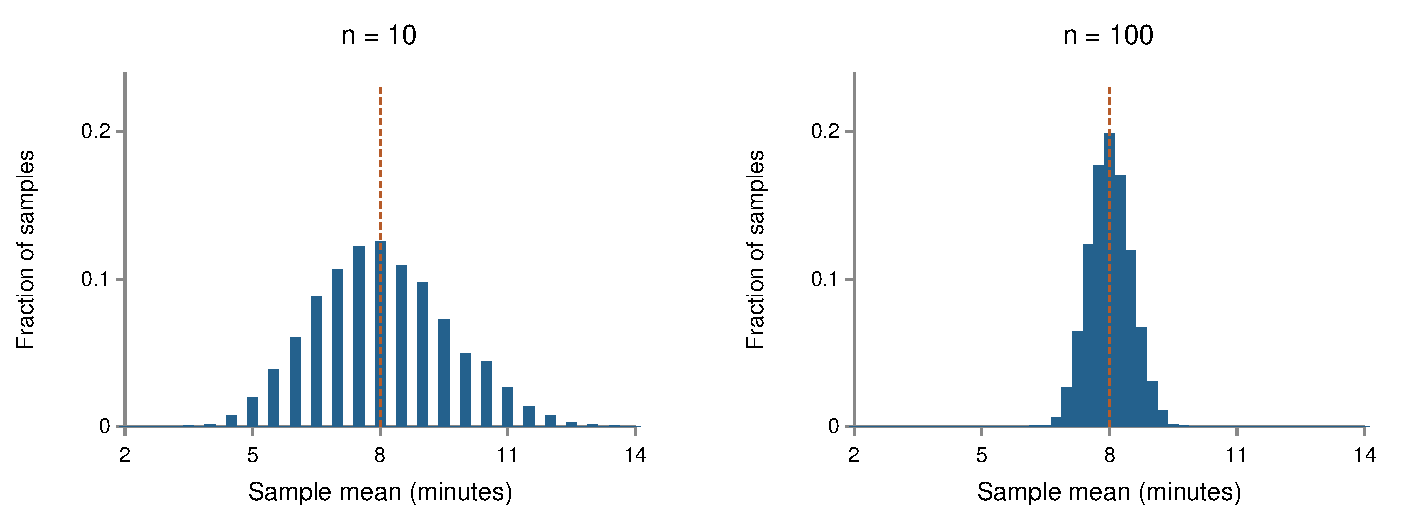
\includegraphics[width=\textwidth]{figures/sampling.pdf}
\caption{Sampling distributions illustrated by 5,000 simulated sample
means at each sample size, from the same discrete waiting model. Each
panel uses the same horizontal scale. Larger independent samples produce
means more tightly concentrated around the model mean of eight minutes.}
\label{fig:ds-sampling}
\end{figure}

For independent observations from a common distribution with variance
$\sigma^2$, the mean has
\[
 \mathbb E[\bar X]=\mu,\qquad
 \operatorname{Var}(\bar X)=\frac{\sigma^2}{n}.
\]
Indeed, averaging preserves the expectation, while independence makes the
variances of the observations add. Dividing their sum by $n^2$ gives the
second formula. The standard deviation of an estimator is its
\emph{standard error}; here it is $\sigma/\sqrt n$.
In our model it is about $1.61$ minutes for $n=10$ and $0.51$ minutes for
$n=100$. Multiplying the sample size by four halves the standard error.
It does not eliminate systematic errors in measurement or selection.

Repeated observations may fail to be independent. Ten waits during the
same equipment breakdown can be much more alike than ten visits spread
across a month. The formula above is a result under assumptions, not a
universal reward for collecting more rows.

\section{Estimation: an answer with an indication of uncertainty}
\label{sec:ds-estimation}
Suppose 60 of our 100 sampled students say they would use the evening bus.
The sample proportion is $\hat p=60/100=0.60$. This estimates the population
proportion, but another random sample could give a different answer.

For independent yes/no responses with common probability $p$, represent
yes by 1 and no by 0. Each observation has mean $p$ and variance $p(1-p)$.
The sample proportion is their mean. Substituting $\hat p$ for the unknown
$p$ gives the approximate standard error
\[
 \widehat{\operatorname{SE}}(\hat p)
 =\sqrt{\frac{\hat p(1-\hat p)}{n}}
 =\sqrt{\frac{0.6(0.4)}{100}}\approx 0.049.
\]
A commonly used large-sample approximation gives a 95\% confidence interval
by taking the estimate plus or minus about $1.96$ standard errors:
\[
 0.60\pm1.96(0.049)\approx[0.504,0.696].
\]
This suggests reporting about 60\%, with sampling uncertainty of roughly
10 percentage points in either direction, rather than presenting 60\%
as an exact population fact.\footnote{This simple normal approximation is
not reliable for very small samples or proportions near zero or one.
Sampling 100 distinct students from a population of 2,000 also introduces
a finite-population correction: the standard error is multiplied by
$\sqrt{(2000-100)/(2000-1)}\approx 0.975$. Ignoring that small correction here
slightly widens the interval. Neither version accounts for nonresponse
or inaccurate answers.}

What does 95\% mean? Under the sampling assumptions, if we repeatedly drew
samples and constructed intervals by this procedure, approximately 95\%
of those intervals would contain the fixed population proportion. It does
not mean that 95\% of students lie in the numerical interval. Nor does it
say that the particular interval has a 95\% probability of containing a
parameter in this frequentist interpretation: the parameter is fixed,
and the procedure's intervals vary.

A useful conclusion states both the estimate and what it estimates:
expressed intention under the proposed service description. Actual bus
use may differ. Statistical precision does not remove that distinction.

\subsection{Estimating an area by sampling points}
\label{sec:ds-area}
\paragraph{The problem.}
How could we estimate the area inside a curved boundary if testing whether
a point lies inside is easy, but a direct area calculation is difficult?

As in \QRMTprevious{chap:geometry}{Chapter}{the geometry chapter},
we represent a region using coordinates and distances. Here we use that
representation to turn an area question into a sampling question.
Start with a familiar case. Choose $(U,V)$ uniformly from the unit square,
with the two coordinates independent. The point lies in its quarter disk
exactly when $U^2+V^2\leq1$. Because selection is uniform, the probability
of this event equals its area divided by the square's area: $\pi/4$.
If $K$ of $N$ independently sampled points pass the test, then
\[
 \widehat\pi=4\frac KN
\]
is an estimate of $\pi$. This is not a practical competitor to specialised
algorithms for computing $\pi$, but it demonstrates a method that also
works for less familiar regions. Figure~\ref{fig:ds-area} shows one such
sample and distinguishes the points that pass the test.

\begin{figure}[htbp]\centering
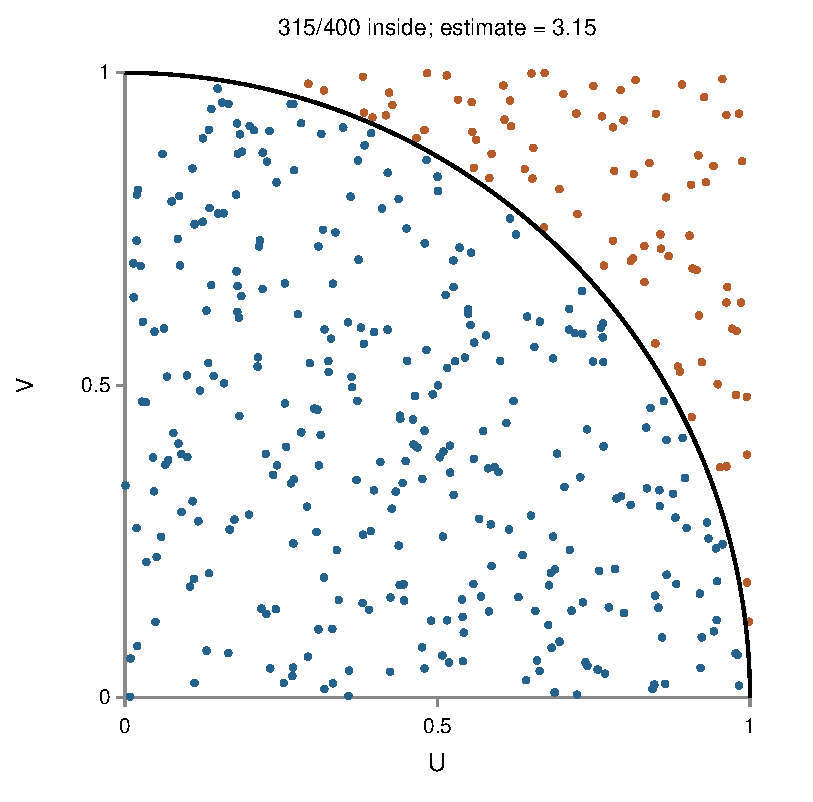
\includegraphics[width=0.58\textwidth]{figures/area.pdf}
\caption{Four hundred uniformly sampled points. The proportion inside the
quarter disk estimates its fraction of the square's area. The result
varies with the sample; the curved boundary itself is fixed.}
\label{fig:ds-area}
\end{figure}

We follow the method of deriving an invariant from a desired final state,
used in \QRMTprevious{sec:imperative-invariants}{Section}{the discussion of
loop invariants in the imperative computation chapter}.
At termination, we want $K$ to count the hits among exactly $N$ sampled
points. Generalise this statement to an intermediate stage: after $i$
repetitions, $K$ counts exactly the hits among those $i$ points, with
$0\leq K\leq i$. This is the invariant we maintain. The quantity $N-i$
decreases by one at each repetition until it reaches zero.
The resulting procedure is:
\begin{quote}
\begin{minipage}{\linewidth}
\textbf{Given:} a positive integer $N$.\\
Set $i=0$ and $K=0$.\\
While $i<N$:\\
\hspace*{1em}Generate independent uniform coordinates $U,V$ in $[0,1]$.\\
\hspace*{1em}If $U^2+V^2\leq1$, replace $K$ by $K+1$.\\
\hspace*{1em}Replace $i$ by $i+1$.\\
Return $4K/N$.
\end{minipage}
\end{quote}
Initially no points have been sampled and $K=0$, so the invariant holds.
Each repetition counts precisely the new hit, if there is one, and then
increases $i$. At termination $i=N$, so the returned quantity is the
intended estimate. This proves correctness as a computation of an
estimate; it does not prove that the estimate equals $\pi$. Its accuracy
is a separate probabilistic question.

With $p=\pi/4$, the estimator's standard error is
$4\sqrt{p(1-p)/N}$. Again, reducing random error by a factor of two requires
about four times as many samples. To estimate an irregular region, enclose
it in a rectangle of known area, sample uniformly in the rectangle, and
multiply the fraction of hits by the rectangle's area.

\section{Curve fitting: describing a relationship}
\label{sec:ds-fitting}
\paragraph{The problem.}
Can the number of customers ahead of us help predict our cafeteria wait?
Suppose we record five further visits during the lunch rush, under
comparable staffing conditions. These are a separate, deliberately simple
dataset; they are not the ten visits used earlier.
\begin{center}
\begin{tabular}{c rrrrr}
\toprule
Customers ahead, $x$ & 2 & 4 & 6 & 8 & 10\\
Wait $y$ (minutes) & 12 & 15 & 19 & 20 & 24\\
\bottomrule
\end{tabular}
\end{center}
Plotting each row pair as a point $(x_i,y_i)$ reveals a roughly increasing
relationship. A simple model is a straight line
\[
 \widehat y=a+bx.
\]
Its slope $b$ has units of minutes per additional customer ahead; its intercept $a$ has
units of minutes. The model might suggest a fixed preparation delay plus a queueing
component. That interpretation is a hypothesis about the mechanism,
not something established by fitting a line.

For a given line, the \emph{residual} is
$e_i=y_i-(a+bx_i)$: observed wait minus predicted wait. Choose $a,b$ to
minimise the sum of squared residuals,
\[
 Q(a,b)=\sum_{i=1}^{n}\bigl(y_i-a-bx_i\bigr)^2.
\]
These are vertical distances in the plot, because the task predicts waiting time
from queue length. Perpendicular distances would define a different problem.

\subsection{Finding the line without guessing}
For any fixed $b$, the best $a$ is the mean of the quantities $y_i-bx_i$,
by the squared-distance property of the mean. Thus $a=\bar y-b\bar x$.
Put $u_i=x_i-\bar x$ and $v_i=y_i-\bar y$. Substituting and expanding gives
\[
 Q=\sum_i v_i^2-2b\sum_i u_iv_i+b^2\sum_i u_i^2.
\]
When the $x_i$ are not all equal, completing the square shows that the
minimum occurs at
\[
 b=\frac{\sum_i(x_i-\bar x)(y_i-\bar y)}
         {\sum_i(x_i-\bar x)^2},\qquad a=\bar y-b\bar x.
\]
For our data, $\bar x=6$, $\bar y=18$, the numerator is 58, and the
denominator is 40. Hence
\[
 \widehat y=9.3+1.45x.
\]
The residuals are $-0.2,-0.1,1,-0.9,0.2$ minutes, with squared sum $1.90$.
The prediction at $x=6$ is 18 minutes; the observed wait was 19.
A fitted line summarises a pattern without passing through every point.
Figure~\ref{fig:ds-fit} displays the fitted line and the residuals; the
second panel lets us inspect the errors separately from the overall trend.

\begin{figure}[htbp]\centering
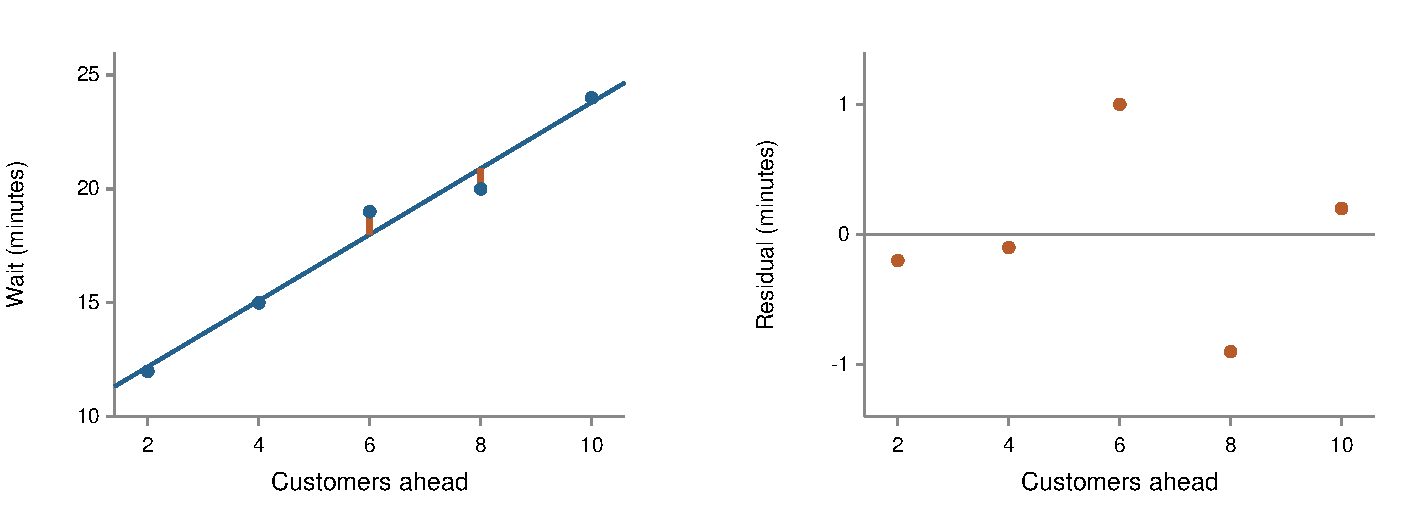
\includegraphics[width=\textwidth]{figures/fit.pdf}
\caption{Left: the least-squares line and its vertical residuals.
Right: the same residuals plotted against queue length. Residual plots help
reveal systematic patterns that a fitted line may conceal. Five points
are far too few to establish a dependable prediction rule.}
\label{fig:ds-fit}
\end{figure}

The formula also specifies a computation. One pass through the data finds
$\bar x,\bar y$; another accumulates the two centred sums. Each pass takes
a number of arithmetic operations proportional to $n$: an $O(n)$ count
in the terminology of \QRMTprevious{sec:algorithms-complexity}{Section}{the
discussion of complexity in the algorithms chapter}. We need not search
through a large collection of possible lines. The mathematical derivation
has supplied a procedure.

\subsection{A close fit is not the same as a good prediction}
A polynomial of degree at most four can pass exactly through these five
points, since their queue lengths are distinct. Zero training error might
sound ideal, but the resulting curve can behave badly between points or
outside the observed range. This is \emph{overfitting}: following the
particular sample too closely to predict new observations well.
In Figure~\ref{fig:ds-overfit}, compare the exact-fitting polynomial
with the straight line, especially beyond the observed range.

\begin{figure}[htbp]\centering
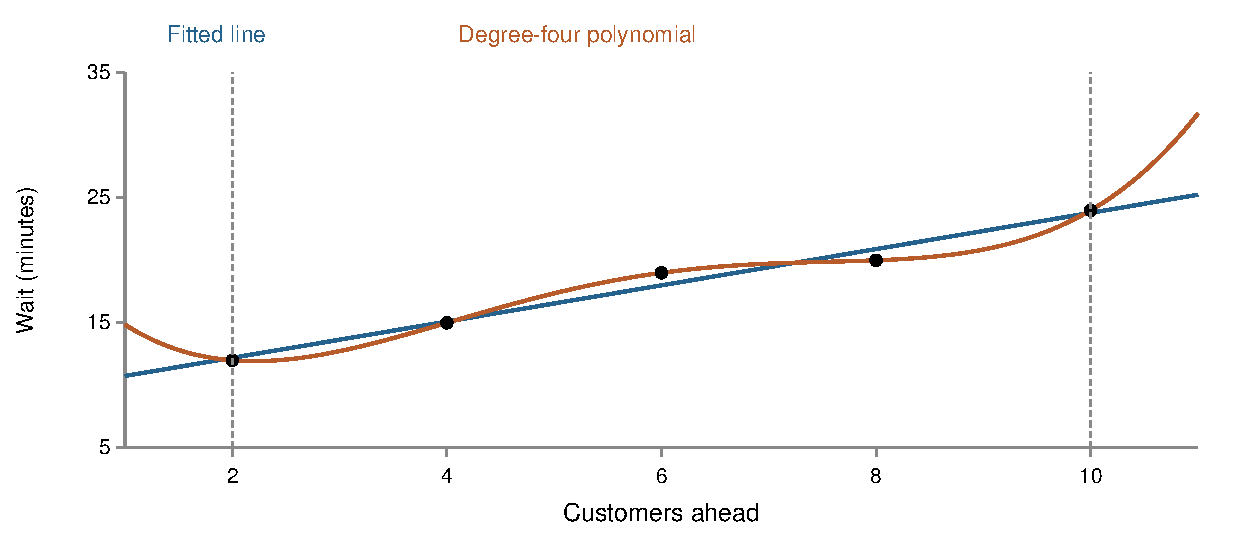
\includegraphics[width=0.8\textwidth]{figures/overfit.pdf}
\caption{The interpolating polynomial matches all five observations, but
bends sharply near the ends and beyond them. The dashed vertical lines
mark the observed queue-length range. A perfect fit to these points does not
decide which model predicts future cafeteria waits better.}
\label{fig:ds-overfit}
\end{figure}

Reserve some observations for checking predictions rather than fitting the
model. Compare predicted and observed values on these \emph{held-out} data.
If model choices are repeatedly adjusted using that check, it becomes part
of the fitting process; a final test requires fresh data. For future-time
prediction, testing on later observations is often more appropriate than
randomly mixing earlier and later records.

Predicting at an unobserved queue length within the measured range is
\emph{interpolation}; predicting beyond it is \emph{extrapolation}.
Neither is automatically reliable, but extrapolation asks the pattern to
continue where it has not been observed. The intercept 9.3 should not be
reported as a measured wait when nobody is ahead in the queue.

\section{Inference: could chance explain the difference?}
\label{sec:ds-inference}
\paragraph{The problem.}
A new set of written instructions is intended to help people solve a
puzzle. How could we investigate whether it improves performance?

Recruit 40 participants and arrange them into 20 pairs using relevant
prior experience, before assigning instructions. Within each pair, use an
independent fair random choice to give one participant the new instructions
and the other the old instructions. Everyone attempts the same task under
the same conditions. Suppose there are no tied scores, and the participant
with the new instructions scores higher in 15 of the 20 pairs.

\paragraph{What is a null hypothesis?}
A \emph{null hypothesis}, denoted $H_0$, is a specified claim used as a
reference for assessing the observations. It often expresses ``no effect''
or ``no difference'', but its content must be stated for the particular
problem. Here it is the claim that changing the instructions would change
\emph{nobody's} score. This is stronger than saying that positive and
negative effects average to zero.

We ask what results would be plausible if $H_0$ were true, under the
actual random-assignment procedure. An unusually large number of wins
for the new instructions would count against that reference claim, in
the direction of our proposed improvement. This reasoning does not start
by assuming that $H_0$ is known to be true. Nor does failing to find an
unusual result establish that it is true: a study may contain too little
information to detect an effect.\footnote{See OpenStax,
\emph{Introductory Statistics 2e},
\href{https://openstax.org/books/introductory-statistics-2e/pages/9-1-null-and-alternative-hypotheses}
{Section 9.1, ``Null and Alternative Hypotheses''}. Our example uses a
no-effect claim for every participant, allowing an exact comparison based
on the random assignment.}

Random assignment makes the comparison informative: under the
\emph{null hypothesis} that changing instructions affects nobody's score,
the two scores in each pair would stay fixed when the instruction labels
are swapped. Either member is equally likely to receive the new version.
Consequently, under this hypothesis, the number $W$ of pairs won by the
new version behaves like the number of heads in 20 independent fair
coin tosses.

There are $2^{20}$ equally likely assignment patterns. Exactly
$\binom{20}{k}$ put the new label on the higher score in $k$ pairs. Therefore
\[
 P(W=k)=\binom{20}{k}2^{-20},\qquad k=0,\ldots,20.
\]
This is a \emph{binomial distribution}, here with 20 trials and success
probability $1/2$. The model provides a reference against which the
observed result can be compared.

If we specified in advance that the question was whether the new version
improves scores, the probability of a result at least as favourable is
\[
 P(W\geq15)=\sum_{k=15}^{20}\binom{20}{k}2^{-20}
 =\frac{21700}{1048576}\approx 0.0207.
\]
This is a one-sided \emph{$p$-value}: the probability, under the null
hypothesis and the assignment procedure, of a result at least this extreme
in the specified direction. If either improvement or deterioration was
the question, the symmetric two-sided probability is about $0.0414$.
We must not choose a direction after inspecting the result merely to
obtain the smaller number. Figure~\ref{fig:ds-inference} highlights the
upper tail whose probabilities we have just added.

\begin{figure}[htbp]\centering
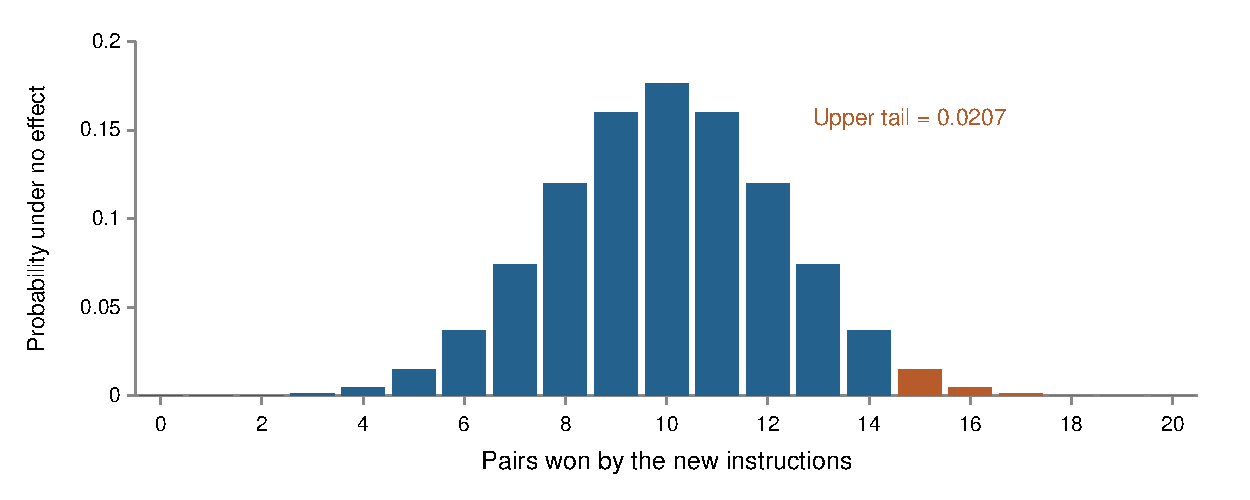
\includegraphics[width=0.85\textwidth]{figures/inference.pdf}
\caption{The reference distribution under no effect of instructions.
The highlighted upper tail is the one-sided probability of 15 or more
wins for the new instructions. This distribution is about the random
assignment, not a distribution of individual puzzle scores.}
\label{fig:ds-inference}
\end{figure}

A small $p$-value says that the result is unusual under this null model.
It is not the probability that the null hypothesis is true, and it does
not measure how large or educationally useful the improvement is.
We should also examine the score differences and their uncertainty.
A tiny gain in many pairs and a large gain in many pairs can produce the
same win count.

Random selection and random assignment do different jobs. Selection helps
us reason from a sample to a population. Assignment helps us compare
interventions without systematically giving one to participants who would
otherwise perform better. A randomly assigned experiment on volunteers
can support a causal comparison for those participants while leaving
questions about other populations unresolved.

Finally, analysing many outcomes until one looks unusual changes the
meaning of the calculation. Under a valid null model, a test with a 5\%
false-positive rate occasionally flags a difference even when there is
none. Trying many such tests creates many opportunities. Recording the
main question and analysis before observing outcomes helps keep the
comparison honest.

\subsection{From this experiment to a randomised controlled trial}
\label{sec:ds-rct}
Our instruction experiment is a small \emph{randomised controlled trial}
(RCT). ``Randomised'' refers to assignment of the intervention; ``controlled''
means there is a comparison condition. The control need not receive
nothing: here it receives the old instructions. The same design idea can
compare teaching methods, public programmes, or ways of providing a service.

The difficulty in evaluating an intervention is that we cannot observe
both outcomes for the same person on the same occasion: their result with
the new instructions and their result with the old ones. The unobserved
alternative is called a \emph{counterfactual}. Random assignment creates
groups whose comparison can estimate an average effect, rather than
requiring both outcomes for every individual.

Randomisation makes differences in prior characteristics unsystematic
across possible assignments; it does not make the realised groups exactly
identical. In our paired design, we compare the scores within each pair
and can average those differences to estimate the effect for the study
participants. The win count used above answers a different, narrower
question about which instruction version tends to win within pairs.

A credible trial specifies the intervention, comparison, outcome, and
analysis before results are examined. It also follows what happened:
did participants use their assigned instructions, did some leave, and
did people share instructions across groups? Analysing people according
to their assigned group preserves the original random comparison; if
some do not follow the assignment, this estimates the effect of assignment
or offering the intervention, which may differ from the effect of using it.

Participation and allocation must be ethically acceptable. Randomisation
also does not guarantee that the result transfers to a different population
or setting. These limits make an RCT a useful design for suitable questions,
not an automatic answer to every causal question.\footnote{For an accessible
introduction, see J-PAL,
\href{https://www.povertyactionlab.org/resource/introduction-randomized-evaluations}
{``Introduction to randomized evaluations''}.}

\section{Clustering: discovering groups in observations}
\label{sec:ds-clustering}
\paragraph{The problem.}
The cafeteria records the numbers of meals and drinks sold in successive
ten-minute periods. Are there recognisable patterns of activity, without
specifying in advance which periods belong to which type?

Represent a period by a point $(x,y)$, where $x$ counts meals and $y$
counts drinks. Consider six observations:
\[
 (1,2),\ (2,1),\ (3,3),\ (7,7),\ (8,6),\ (9,8).
\]
The plot suggests two groups. \emph{Clustering} means grouping observations
according to a chosen notion of similarity. Here we use ordinary Euclidean
distance in the plane, and choose to seek two clusters. This is called
\emph{unsupervised learning}: no correct group labels have been supplied.

\subsection{Represent each group by a centre}
For a fixed group, the point that minimises the sum of squared distances
to its members is its coordinatewise mean. To see why, write a proposed
centre as $(a,b)$. The objective is
\[
 \sum_i\bigl[(x_i-a)^2+(y_i-b)^2\bigr].
\]
The two coordinates can be minimised separately, using the geometric
property of the mean from Section~\ref{sec:ds-summaries}. The first three
observations have centre $c_1=(2,2)$ and the last three have centre
$c_2=(8,7)$.

Usually we do not know the groups beforehand. A common procedure,
\emph{$k$-means}, alternates two simple operations:
\begin{enumerate}
\item Choose $k$ initial centres; here $k=2$.
\item Assign each observation to its nearest centre, resolving ties by a
fixed rule.
\item Replace each centre by the mean of its assigned observations. If a
centre has no assigned observations, retain it for this version of the
procedure.
\item Repeat the assignment and update until memberships no longer change,
or a stated iteration limit is reached.
\end{enumerate}
Assigning to the nearest centre cannot increase the total squared distance
for fixed centres. Replacing a centre by the mean cannot increase it for
fixed groups. Thus each stage improves or preserves the same objective.
This does not guarantee the best possible partition: different starting
centres can lead to different results. Starting our example at $(1,2)$
and $(9,8)$ gives the two groups above after the first assignment and the
two stated means after the update.

\subsection{The Voronoi regions reappear}
Once the centres are fixed, every point in the plane has a nearest centre.
The resulting regions are exactly the Voronoi regions encountered in the
geometry chapter
(\QRMTprevious{sec:geometry-voronoi}{Section}{the section on Voronoi regions}).
Their boundaries are perpendicular bisectors of the
segments joining centres. For our two centres, the boundary satisfies
\[
 (x-2)^2+(y-2)^2=(x-8)^2+(y-7)^2,
 \quad\text{or}\quad 12x+10y=105.
\]
A new period with counts $(5,4)$ is nearer $c_1$: its squared distances
are 13 and 18. The geometric rule therefore assigns it to the first group.
Figure~\ref{fig:ds-clustering} shows the centres, their boundary, and
the position of this new point.

\begin{figure}[htbp]\centering
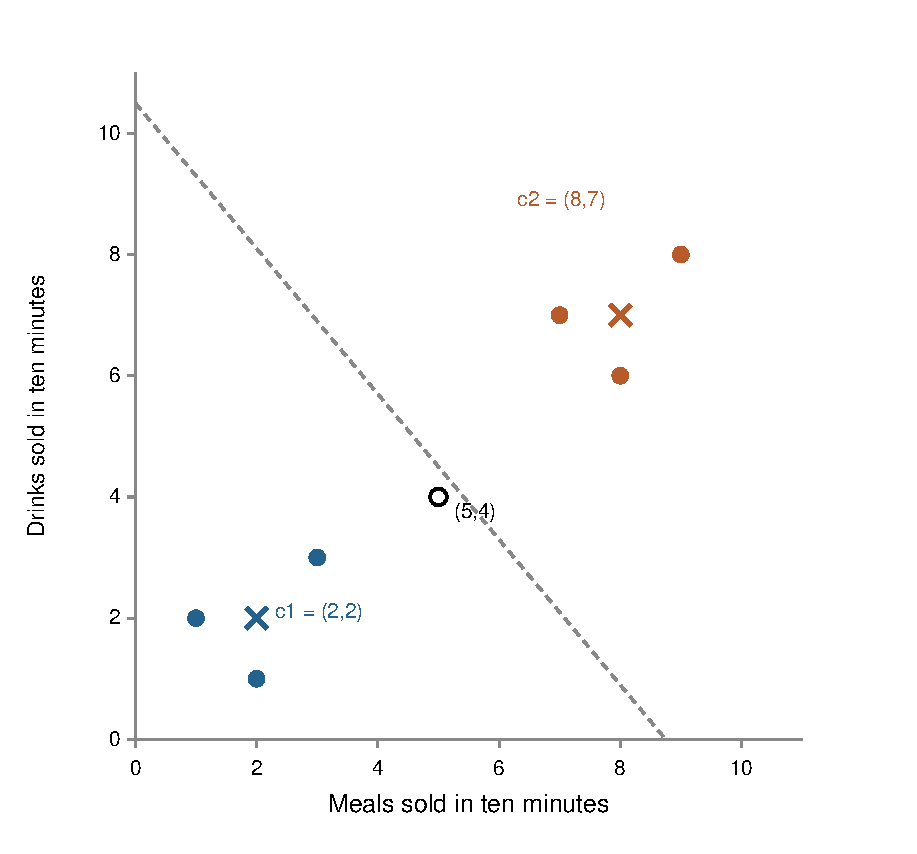
\includegraphics[width=0.76\textwidth]{figures/clustering.pdf}
\caption{Two clusters of cafeteria activity. Crosses mark their mean
centres; the dashed perpendicular bisector separates their Voronoi regions.
The unfilled point $(5,4)$ would be assigned to the first centre.
These are hypothetical observations, not discovered population types.}
\label{fig:ds-clustering}
\end{figure}

The interpretation requires care. Asking for two clusters will produce
two groups even when the data have no convincing separation. The groups
here suggest quieter and busier periods; they do not establish two natural
kinds of customers. Changing the variables, their relative scales, or $k$
can change the answer. If one coordinate measured rupees and another
counted meals, numerical distances would depend strongly on the units.
Scaling is therefore a modelling decision. Clustering can suggest questions
to investigate; it does not supply a causal explanation of the groups.

\section{Classification: predicting a known category}
\label{sec:ds-classification}
\paragraph{The problem.}
At the moment a customer joins the queue, can we predict whether their
wait will exceed ten minutes?

For past visits we record customers ahead, $q$, and active servers, $s$,
at arrival. We also record the eventual outcome: \emph{long} if the wait
exceeds ten minutes, and \emph{short} otherwise. These outcome categories
are \emph{labels}. Unlike clustering, \emph{classification} uses examples
with known labels to build a rule for predicting the label of a new case.
It is a form of \emph{supervised learning}. The inputs used for prediction
are often called \emph{features}.

Suppose a candidate rule, chosen using training observations, is
\[
 \widehat{\text{label}}(q,s)=
 \begin{cases}
 \text{long},&q>3s,\\
 \text{short},&q\leq3s.
 \end{cases}
\]
This rule is illustrative, not a law of queues. Its \emph{decision boundary}
is the line $q=3s$. With two servers and eight people ahead it predicts
long; with three servers and eight people ahead it predicts short.
Figure~\ref{fig:ds-classification} compares the regions predicted by
this rule with the known labels of ten training observations.
The completed waiting time must not be an input: that would reveal the
answer rather than predict it from information available on arrival.

\begin{figure}[htbp]\centering
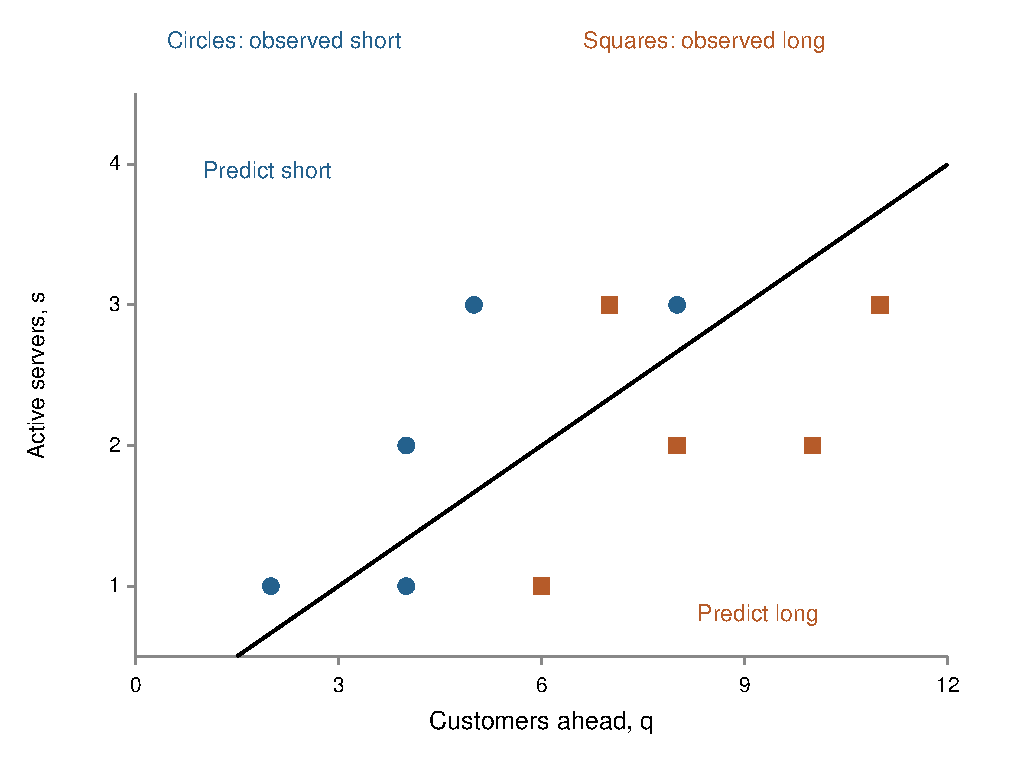
\includegraphics[width=0.76\textwidth]{figures/classification.pdf}
\caption{A candidate classification rule. Symbols show known labels for
ten illustrative training visits; the line separates the rule's two
predictions. Some observations lie on the wrong side for their labels.
Unlike a Voronoi partition in clustering, this boundary is used to predict
categories specified before fitting the rule.}
\label{fig:ds-classification}
\end{figure}

How well does the rule work? Evaluate it on later visits that were not
used to choose it. Suppose a separate test set of 20 visits gives:
\begin{center}
\begin{tabular}{lrr}
\toprule
 & Actually long & Actually short\\
\midrule
Predicted long & 8 & 4\\
Predicted short & 2 & 6\\
\bottomrule
\end{tabular}
\end{center}
This is a \emph{confusion matrix}. The rule is correct on $8+6=14$ visits,
so its accuracy is $14/20=0.70$. But the two errors have different meanings:
four false alarms predict a long wait that does not occur; two missed
long waits give misleading reassurance.

If long waits are the condition of interest, \emph{precision} is the
fraction of predicted long waits that actually are long, here
$8/(8+4)=2/3$. \emph{Recall} is the fraction of actual long waits that are
identified, here $8/(8+2)=0.80$. If long waits were very rare, always
predicting short could achieve high accuracy while detecting none.
The useful measure depends on the decision and the costs of the errors.

Moving the threshold changes the trade-off: a rule that predicts long
more readily generally catches more long waits while producing more
false alarms. Choose such changes using training or validation data;
reusing the final test set to adjust the threshold spoils its independent
check. Twenty test visits also give an uncertain estimate of performance.
A change in staffing or ordering practices may change future performance.

Clustering asks what groups the chosen features suggest. Classification
asks how well those features predict an already specified category.
Neither a visually neat partition nor a good training score is enough:
the question, the observations, and the intended use still have to agree.
\footnote{For further discussion of the distinction, see Penn State,
\href{https://online.stat.psu.edu/stat555/node/17/}{STAT 555, ``Classification''}.}

\section{What exactly does the evidence justify?}
\label{sec:ds-validity}
The calculations above leave several questions to be asked about the
connection between observations and conclusions. We can organise these
questions using three kinds of \emph{validity}. They are useful distinctions,
not three boxes whose labels automatically settle an argument.

\subsection{Construct validity: did we measure the intended idea?}
A \emph{construct} is an idea we want to investigate, such as understanding,
well-being, or convenience. The recorded variable is an operational way
of measuring it. The link between the two needs an argument.

In the instruction experiment, a puzzle score measures performance on a
particular task. If we claim the instructions improve ``understanding'',
we should ask whether success could instead reflect memorised steps,
familiarity with the question, or faster reading. Testing transfer to a
new problem and asking for explanations would provide different evidence.
Similarly, saying one would use a bus is not the same measurement as
actually boarding it, and counting clicks is not a direct measure of
learning. More observations of the same proxy do not repair a poor link
to the intended idea.

\subsection{Internal validity: does the comparison support the explanation?}
Suppose users of the new instructions were volunteers who chose them,
while everyone else used the old version. A difference in scores could
reflect prior motivation or experience. These alternative explanations
threaten the causal conclusion. A \emph{confounder} is a factor that
influences both which condition people receive and the outcome.

Random assignment addresses systematic allocation differences. It does
not prevent every problem: participants may exchange instructions,
leave the study at different rates, or be scored differently by someone
who knows their assignment. Fair comparison also requires attention to
implementation and measurement.

The cafeteria data illustrate a different limit. Queue length predicts
waiting time, but the fitted line alone does not prove that each additional
customer ahead causes exactly 1.45 extra minutes. Longer queues might
coincide with more complicated orders or a shortage of staff. Prediction and causal explanation are
different tasks even when they use the same table.

\subsection{External validity: where else should the conclusion apply?}
Would the instruction result hold for younger learners, another language,
or a much harder task? Would the waiting-time model survive an examination
week? These are questions about extending a conclusion to new people,
settings, or times.

The appropriate population must be stated. A carefully run experiment can
be informative within its setting without justifying every extension.
Broader sampling, repetition in different settings, and an account of why
the mechanism should remain similar all strengthen a generalisation.
The extrapolation of a fitted curve is one mathematical version of this
wider problem.

\paragraph{Putting the questions together.}
Consider the claim, ``The new instructions improve students' mathematical
understanding.'' The score must represent understanding; the comparison
must isolate the effect of instructions; and the participants and tasks
must support the proposed scope. A precise estimate or a small $p$-value
cannot, by itself, establish any of these three links.

\section{A small investigation from start to finish}
\label{sec:ds-investigation}
Choose a modest question, such as predicting cafeteria waiting time from
the number of customers ahead. Define the starting and finishing events,
record queue length and waiting time in stated units, and decide which
conditions belong in the investigation. Use consent where observations concern other people,
and avoid collecting identities when they are unnecessary.

Plan how visits and occasions will be selected before collecting results.
Plot the observations, describe their variation, and try a simple prediction
rule. Keep some later visits for checking it. Compare errors, look for
patterns associated with time of day or staffing, and explain why any
revised model is worth the additional complexity.

Report enough of the procedure that another group could repeat it: the
question, observations, selection method, calculations, and limits of the
conclusion. Save the original data separately from corrections, together
with the reasons for those corrections. An unexpected result is a reason
to examine the model and measurements, not to silently discard inconvenient
observations.

\paragraph{From evidence to judgement.}
Data become evidence through a question, a method, and an argument about
what the observations support. Evidence can help us understand a situation,
but choosing what to do also involves purposes, values, practical constraints,
and the people affected. In discussing the place of randomised controlled
trials in public policy, Jean Dr\`eze offers a useful reminder:

\begin{center}
\begin{minipage}{\textwidth}
\begin{minipage}[c]{0.24\textwidth}
\centering

\includegraphics[width=0.88\linewidth]{images/dreze.jpeg}
\end{minipage}\hfill
\begin{minipage}[c]{0.71\textwidth}
\itshape
``evidence involves more than RCTs, understanding more than evidence,
and policy more than understanding.''\\[7pt]
\normalfont ---Jean Dr\`eze\\[4pt]
\small \href{https://www.ideasforindia.in/topics/miscellany/evidence-policy-and-politics}
{``Evidence, policy, and politics''}, \emph{Ideas for India},
3 August 2018; excerpt from the concluding sentence.\\[4pt]
\scriptsize Photograph: \href{https://www.ideasforindia.in/profile/jean}
{Jean Dr\`eze's contributor profile, Ideas for India}.
\end{minipage}
\end{minipage}
\end{center}

\section*{Problems}
\begin{enumerate}
\item For the ten waiting times in Section~\ref{sec:ds-summaries}, calculate
the mean squared deviation and its square root. Replace 24 by 9 and
recalculate the mean and median. Explain which changes more and why.
\item Construct the empirical probability distribution of those ten waits.
Find $P(X\leq4)$, $P(X>5)$, and $\mathbb E[X]$. Explain why this distribution
does not, by itself, determine the probability of a long wait tomorrow.
\item A table gives probabilities $0.2,0.3,0.4$ for the only possible values
$0,1,2$. Explain why it is not a probability distribution. Give two different
ways to repair the table, stating what you change.
\item For the hypothetical discrete waiting model, verify that
$\mathbb E[X]=8$ and $\operatorname{Var}(X)=26$. Find the smallest allowed
waiting-time value $t$ for which $P(X\leq t)\geq 0.9$.
\item Under the uniform bus-wait model, find the probabilities of waiting
at most three minutes and between six and nine minutes. Explain why a
density has units of inverse minutes while a probability has no units.
\item Two groups each have mean waiting time five minutes. In one group
everyone waits five minutes; in the other half wait zero and half wait ten.
Calculate both variances. Which summary would you report to a person who
cannot wait more than six minutes?
\item A poll asks the first 100 people leaving a library about an evening
bus. Identify the target population, the observed sample, and two reasons
selection might affect the answer. Does increasing this sample to 1,000
necessarily resolve the problem?
\item A college has 1,500 resident and 500 commuting students. A survey
samples 100 from each group. Of these, 40 residents and 80 commuters favour
a service. Calculate the pooled sample proportion and the population-share
weighted estimate. Explain why they differ.
\item A sample mean has standard error two minutes when $n=25$. Assuming
independent observations with unchanged variance, what sample size gives
standard error one minute? What size gives half a minute?
\item Describe a simulation that approximates the sampling distribution
of the mean for the discrete waiting model. Explain why repeatedly copying
one observed sample is not equivalent to drawing fresh independent samples.
\item In a random sample of 400 people, 240 answer yes. Calculate the
approximate standard error and 95\% interval using the formula in
Section~\ref{sec:ds-estimation}. Compare its width with the sample of 100.
State one uncertainty this interval does not capture.
\item Explain the difference between the standard deviation of individual
waits and the standard error of their sample mean. Give their values for
100 independent draws from the discrete waiting model.
\item A random-point area calculation finds 785 hits among 1,000 points
in the unit square. Estimate $\pi$ and its standard error by substituting
$785/1000$ for $p$. Why is the estimate not guaranteed to improve after
every additional point?
\item A region lies inside a rectangle of area 60 square metres. Of 2,000
uniformly sampled points, 730 lie inside. Estimate its area. State the
membership test that would be needed to implement this method for a disk
with centre $(a,b)$ and radius $r$.
\item Prove the counting invariant for the random-point procedure by
induction on the number of repetitions. Explain why this proof does not
establish a numerical error bound for the estimated area.
\item Verify the fitted cafeteria waiting-time line, all five residuals, and their
squared sum. Predict the wait with five and with sixteen customers ahead. Which prediction is
extrapolation, and what extra assumption does it require?
\item Starting with the displayed expression for $Q$ in centred variables,
complete the square to derive the least-squares slope. What goes wrong
when all observed queue lengths are equal?
\item Change the unit of waiting time from minutes to seconds. What happens
to the fitted slope, intercept, and predictions? Explain why units must
accompany numerical coefficients.
\item A model predicts its training data perfectly but performs poorly on
new observations. Give a possible explanation. Why should a final test
set not be repeatedly used to choose the model?
\item In the instruction experiment, verify the upper-tail probability by
adding the six binomial coefficients for $k=15,\ldots,20$. Explain why the
calculation concerns the assignment of labels under the null hypothesis.
\item Compare two experiments in which the new version wins in 15 of 20
pairs. In the first, each win is by one score point; in the second, each
win is by ten points. What does the win-count test treat identically?
What additional information should be reported?
\item Explain why ``the $p$-value is 0.02, so there is a 98\% probability that
the new instructions work'' is not a valid interpretation.
\item A study measures learning by time spent on an educational website.
Discuss one concern about each of construct, internal, and external
validity. Suggest an additional observation or design change for each.
\item Design a small investigation of a cafeteria queue. State the
question, population, variables and units, sampling procedure, one useful
plot, and a method for checking a prediction. Identify the most important
limitation of the conclusion you expect to draw.
\item A sample of ten visits contains no waits longer than 30 minutes.
Explain why its empirical distribution assigns probability zero to this
event, but this does not establish zero population probability. If the
visits were all sampled before lunch, what further problem arises?
\item In the cafeteria model, let $A$ mean ``wait at most five minutes''
and $B$ mean ``wait longer than ten minutes''. Are these events mutually
exclusive? Must their probabilities sum to one? Explain using the outcomes
between them.
\item A survey includes equal numbers of visits from a quiet period and
a busy period, although the busy period accounts for 80\% of all visits.
The two sample mean waits are 3 and 8 minutes respectively. Compute the
unweighted mean and the estimate weighted by the shares of visits.
Which answers the question about a randomly chosen visit?
\item Explain one way in which census information can assist a sample
survey, one error a census can still contain, and one reason a survey
may be preferable for a detailed investigation.
\item Explain why the law of large numbers neither makes a long wait
``due'' after ten short waits nor repairs sampling only at quiet times.
State the quantity that becomes stable and the assumptions needed.
\item In the instruction trial, distinguish ``no effect on anyone'' from
``zero average effect''. Explain why random assignment does not imply
that the two realised groups have exactly the same prior characteristics.
\item For the six cafeteria activity points, verify both cluster centres
and derive their Voronoi boundary. Compute the total squared distance to
the assigned centres, and classify $(5,4)$ by its nearest centre.
\item Start the two-centre procedure at $(1,2)$ and $(9,8)$. Perform one
assignment and one update by hand. Explain why each operation cannot
increase the squared-distance objective, and why that observation alone
does not prove that every initialisation gives the best partition.
\item Using the classification confusion matrix, calculate accuracy,
precision, and recall. If long waits are only 5\% of visits, calculate the
accuracy and recall of always predicting short. Explain why accuracy alone
can be misleading.
\item Would adding the final waiting time as an input make a useful
arrival-time classifier? Explain. Give one feature available on arrival
that could plausibly improve the prediction, and one way its measurement
could vary across days.
\end{enumerate}
